\section{Testovanie}

V~tejto kapitole popisujeme proces testovania
implementovanej aplikácie a~uvádzame výsledky
overenia spoľahlivosti rozpoznávania jednotlivých
gest. Cieľom testovania bolo overiť, či hraničné
hodnoty stanovené v~kapitole~\ref{chapter:gesta}
zabezpečujú spoľahlivú detekciu gest pri ich
opakovanom vykonávaní.

\subsection{Metodika testovania}

Testovanie sme rozdelili do troch fáz, ktoré sa
postupne približujú k~reálnym podmienkam použitia
aplikácie. V~prvej fáze sme overovali úspešnosť
rozpoznania jednotlivých gest pri ich izolovanom
vykonávaní. V~druhej fáze sme testovali kompletné
kompozitné sekvencie zodpovedajúce reálnym scenárom
použitia. V~tretej fáze sme overovali odolnosť
aplikácie voči falošne pozitívnym detekciám
pri bežnej aktivite ruky.

Testovanie prebiehalo v~debug móde Android aplikácie
(viď podsekciu~\ref{app:debug-final}), ktorý umožňuje
vizuálnu kontrolu rozpoznaných gest v~reálnom čase.
Pre každý test bola zaznamenávaná informácia o~tom,
či aplikácia gesto správne rozpoznala, prípadne aký
bol dôvod chybnej detekcie. Testy vykonával jeden
používateľ (autor práce) v~stoji, v~kontrolovanom
prostredí.

\subsection{Testovanie jednotlivých gest}
\label{subsec:test-jednotlive}

V~prvej fáze testovania sme každé gesto vykonali
20-krát v~ideálnych podmienkach (v~stoji, bez
sprievodných pohybov tela, v~neutrálnej polohe ruky
medzi pokusmi). Cieľom bolo overiť spoľahlivosť
detekcie samotného gesta bez vplyvu kontextu.

Pre testovanie gesta \uv{Hand Down} platí špecifický
postup -- toto gesto sa testuje vždy ako návrat
z~iného režimu, keďže v~režime \texttt{WAITING}
už ruka v~neutrálnej polohe je. Hand Down sme preto
testovali v~kombinácii s~aktivačným gestom Rise Arm.

Výsledky úspešnosti rozpoznania jednotlivých gest
sú zhrnuté v~tabuľke~\ref{tab:test-jednotlive}.

\begin{table}[H]
  \centering
  \caption{Úspešnosť rozpoznania jednotlivých gest}
  \label{tab:test-jednotlive}
  \renewcommand{\arraystretch}{1.3}
  \begin{tabularx}{\textwidth}{
      >{\raggedright\arraybackslash}X
      >{\centering\arraybackslash}p{0.15\textwidth}
      >{\centering\arraybackslash}p{0.18\textwidth}
      >{\centering\arraybackslash}p{0.18\textwidth}
    }
    \toprule
    \textbf{Gesto}         & \textbf{Pokusy} & \textbf{Rozpoznané} & \textbf{Úspešnosť} \\
    \midrule
    Rise Arm               & 20              & 18                  & 90,0\%             \\
    \midrule
    Hand Back              & 20              & 16                  & 80,0\%             \\
    \midrule
    Hand Down              & 20              & 20                  & 100\%              \\
    % \midrule
    % Flick                  & 18              & XX                  & XX,X\,\%           \\
    \midrule
    PASIVITA -- červený    & 20              & 17                  & 85,0\%             \\
    \midrule
    PASIVITA -- modrý      & 20              & 18                  & 90,0\%             \\
    \midrule
    NAPOMENUTIE -- červený & 20              & 18                  & 90,0\%             \\
    \midrule
    NAPOMENUTIE -- modrý   & 20              & 19                  & 95,0\%             \\
    \midrule
    TOUCHE                 & 20              & 17                  & 85,0\%             \\
    \midrule
    \textbf{Celkovo}       & \textbf{160}    & \textbf{149}        & \textbf{89,4\%}    \\
    \bottomrule
  \end{tabularx}
\end{table}

Z~výsledkov vyplýva, že priemerná úspešnosť rozpoznania
naprieč všetkými gestami dosahuje 89,4\%, čo považujeme
za uspokojivý výsledok pri testovaní v~kontrolovaných
podmienkach. Najvyššiu spoľahlivosť (100\%) dosiahlo
gesto \uv{Hand Down}, ktoré má jasne definovanú neutrálnu
polohu ruky pri tele a~jeho hraničné hodnoty sa neprekrývajú
so žiadnym iným gestom. Vysokú úspešnosť dosahujú aj gestá
\uv{NAPOMENUTIE -- modrý} (95,0\%) a~\uv{Rise Arm} a~\uv{NAPOMENUTIE
  -- červený} (oba 90,0\%).

Najnižšiu úspešnosť sme zaznamenali pri geste
\uv{Hand Back} (80,0\%), čo zodpovedá očakávaniu vyplývajúcemu
z~návrhu — toto gesto má polohu ruky za chrbtom, ktorá je
mechanicky podobná polohe pri geste \uv{NAPOMENUTIE -- modrý}.

\subsubsection{Analýza chybných detekcií}

Pre detailnejšiu analýzu zlyhaní sme zostrojili
konfuznú maticu, ktorá ukazuje, ako sa jednotlivé
gestá zamieňali pri chybných detekciách. Riadky
predstavujú testované gesto, stĺpce predstavujú
rozpoznané gesto. Hodnoty na diagonále
zodpovedajú úspešným rozpoznaniam, ostatné hodnoty
predstavujú chybné detekcie.

\begin{figure}[H]
  \centering
  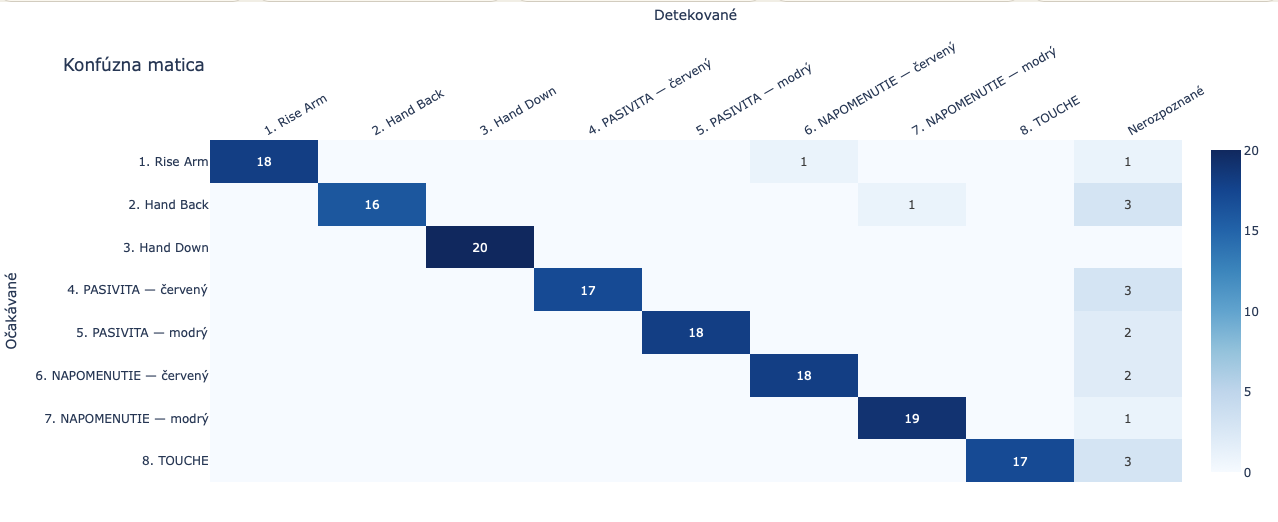
\includegraphics[width=\textwidth]{img/testing/confusion-phase-1.png}
  \caption{Konfúzna matica testovania gest v ideálnych podmienkach}
  \label{fig:confusion-matrix}
\end{figure}
